\emph{This chapter of the report focuses on examination and analysis of current research and development in the field, in order to find out more about the structure of Mobile ad hoc networks (MANETs) and corresponding simulators, how drones can be employed in this field, as well as existing solutions for drone sensor networks. Then, the specific algorithms and characteristics of sensor networks must be researched, as this dictates the core functionality of the project network and how this can be achieved. This chapter will be cover the topics of learning about the current state-of-the-art, and allowing that to influence our design and implementation decisions.}

\section{MANETs}

\subsection{Structure}
It is necessary for a MANET to be capable of self-configuring without an infrastructure, where mobile devices can connect without wires. Given that they are mobile nodes that communicate by forming a network dynamically, they lack a fixed infrastructure or centralised control. Nodes are independent, and the network topology is temporary as each node dynamically self-organises. This means that each device must be a router. Each node must be capable of shifting its organisation, and forwarding packets \cite{jaydipsen2010}. When nodes wish to communicate with one another they can use a variety of different mediums, such as Wi-Fi or radio waves, but they must depend on intermediate nodes to route their data packets in the event that the source and destination are not in range of one another \cite{ramramathanjasonredi2012}.
MANETs may employ a specific network model, or a general approach in which nodes are aware of other nodes in range and their task only. Various methods of forwarding data exist, such as flooding data by broadcasting to all neighbours, or by using predefined metrics to determine the optimal path \cite{jaydipsen2010}. It is in stark contrast to a centralised wireless network, as there are no access points in a managed infrastructure. Forwarding of data is dependent on the basis of network connectivity, so nodes must be able to create and join networks arbitrarily, which requires high adaptability to constant changes in topology. MANET systems must also consider problems such as limited power and storage for each individual node; the network must be fault tolerant such that it can deal with problems such as when connectivity is lost or a node powers down. Energy and power consumption are priority concerns which are directly related to the hardware resources available to each node, and the environment in which the network is deployed \cite{sajshahmina2012}.
POSSIBLE OBLIGATORY PICTURE OF MANET INFRASTRUCTURE

\subsection{Simulations}
\label{simSoft}
Network simulators are software that predict the behaviour of a computer network, making them a popular method for experimentation with a possible model for MANETs due to their ability to cheaply and flexibly model a solution. These simulation tools make it possible to model fault tolerance, scalability, make monitoring easy, and provide reproducibility \cite{stuartkurkowski2005}. It should be noted that there are significant variations in the way that individual simulators operate, which cannot be expressed in terms of accuracy. At best, they can be said to be dependable and realistic, but will have difficulty modelling unpredictable error in a real environment. Simulation events can be split into continuous and discrete simulation, where continuous simulation makes use of analytic models, and so can hardly be applied in practice. Conversely, discrete simulation allows for parallelism for scalability and speed up, as well as developing trace files containing a description of each event that occurred \cite{luchogie2006}. These trace files can then be used to generate a visualisation of the simulation, so they would be preferred for our project (or they will influence how we build our simulation and visualise it). This section gives an overview of the potential solutions available for simulations, and the alternatives to using a simulator.

\subsubsection{ns-2}
ns-2 (network simulator) is a discrete-event network simulator, for research and educational use. Its software infrastructure encourages the development of simulation models which are sufficiently realistic to allow it to be used as a real-time network emulator, and is the basis for many existing real-world implementations \cite{tommasopecorella2016}. In particular, it provides a set of randomised mobility models, including random waypoint, such that the advanced node mobility constitutes a progression towards realistic simulation. ns-2 programs are scripted in OTcl, with some components written in C++ . Despite its popularity, ns-2 suffers for its lack of modularity and inherent complexity, but does provide excellent documentation. It is the predecessor of ns-3, although it has a greater diversity of models given there more years of contributions. ns-2 also allows for visualisation of the simulation through its GUI out.nam with the use of trace files, as shown in figure 8.1 below \cite{luchogie2006}.

\begin{figure}
\centering	
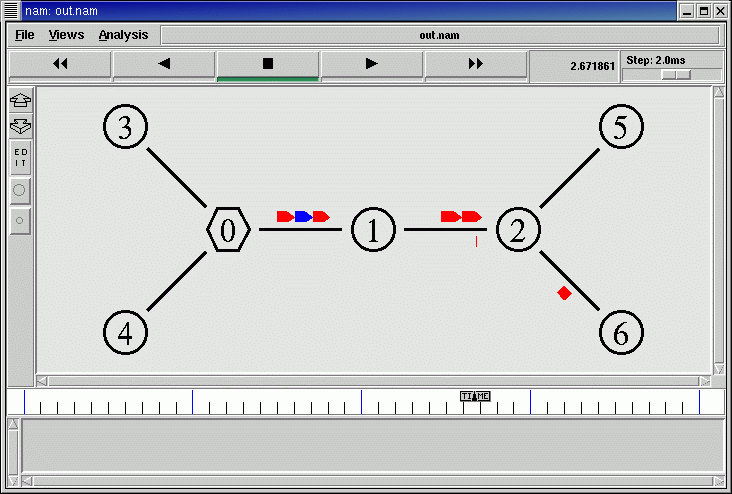
\includegraphics[scale=0.4]{img/outnam}	
\caption{ Visualisation for ns-2 trace files in out.nam}
\end{figure}

\subsubsection{ns-3}
ns-3 is a new software development which followed  ns-2 , focusing its efforts on improving the core architecture, software integration, models, and educational components of ns-2 \cite{ns2006}. ns-3 differs from ns-2 in that it is purely written in C++, with optional Python bindings. New scripts can therefore be written in C++ or in Python. This version is recommended over ns-2 due to features which are not available in the previous version, such as an implementation code execution environment, which allows users to run real implementation code in the simulator. Additionally, it has more detailed models, as well as being actively maintained and developed. ns-3 is not backwards compatible with ns-2; it is an entirely new simulator, with several models which were written in C++ which are already been ported to ns-3 \cite{tommasopecorella2016}. The visualisation platform for ns-3 is the offline animator NetAnim, based on the Qt toolkit.

\begin{figure}
\centering	
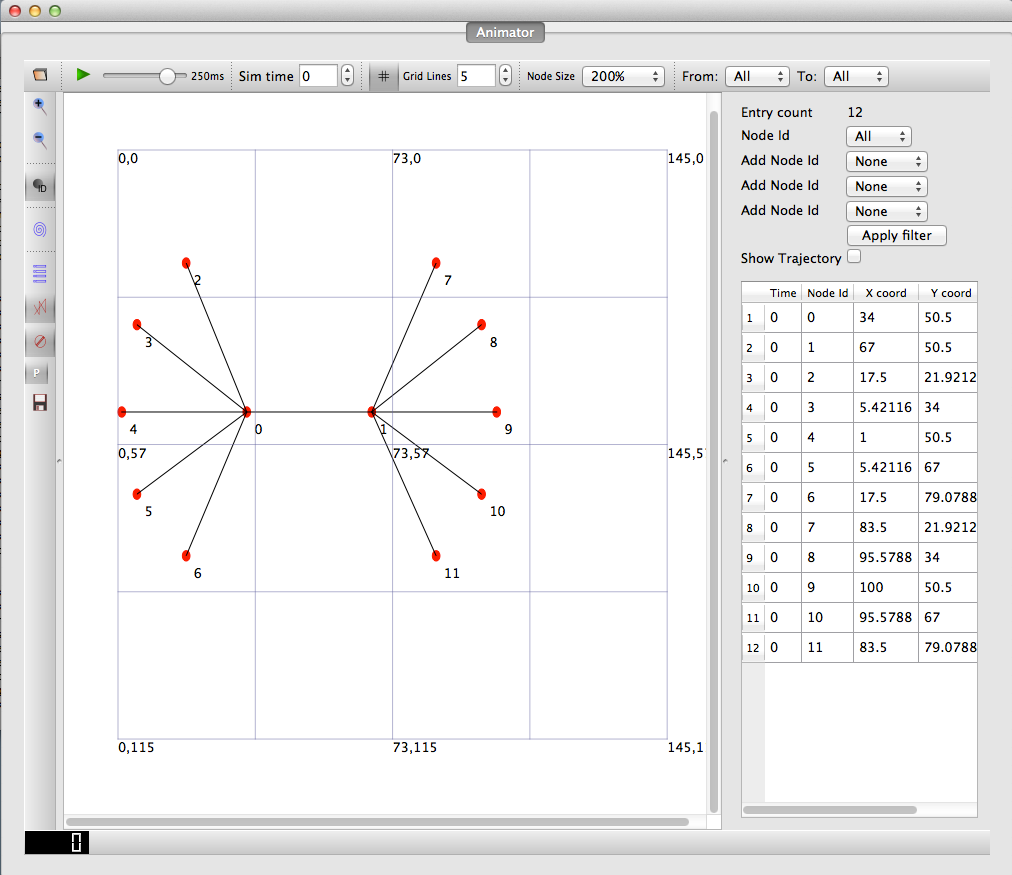
\includegraphics[scale=0.4]{img/netanim}	
\caption{An example of NetAnim simulation animation}
\end{figure}

\subsubsection{GloMoSim}
Short for Global Mobile Information System Simulator, GloMoSim is a network protocol simulation software for parallel simulation of wireless and wired network systems using the parallel programming language PARSEC \cite{zengxiang1998}. It uses a message-based approach to discrete-event simulation, where network layers are represented as objects called entities, which handle events represented by timestamped messages. The library has been designed to be extensible and composable, and its modular implementation enables consistent comparison of protocols at a given layer. While research into parallel simulation is relatively limited, and areas such as signal interference and attenuation are inherently more complicated, there are clear implications for a significant increase in performance in terms of spreading out the simulation overheads, which may outweigh the inherent complexity. The PARSEC Visual Environment (PAVE) has also been developed to support the visual design of GlomoSim event simulations \cite{luchogie2006}.

\begin{figure}
\centering	
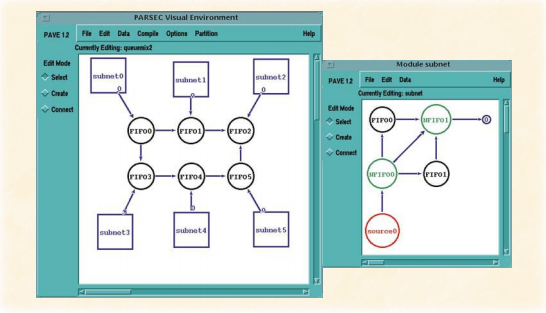
\includegraphics[scale=0.4]{img/pave}	
\caption{Example output from the PARSEC Visual Environment}
\end{figure}

\subsubsection{OMNet++}
OMNet++ is an extensible, modular, component-based C++ simulation library and framework, primarily for building network simulators \cite{omnet2016}. This includes wired and wireless communication networks for sensor networks, ad hoc networks, Internet protocols, and so on. OMNet++ is not a network simulator in and of itself, but provides a wide range of tools and extensions, including an Eclipse-based IDE (Integrated Development Environment). It provides a component architecture for models; components are programmed in C++ and then assembled into larger components and models using a high-level language (NED) which also has GUI support. OMNet++ was designed for the general use case, as opposed to being a specialised simulator, and its modular architecture allows for the simulation kernel (and models) to be easily integrated into wider systems \cite{varga2008}. 

\begin{figure}
\centering	
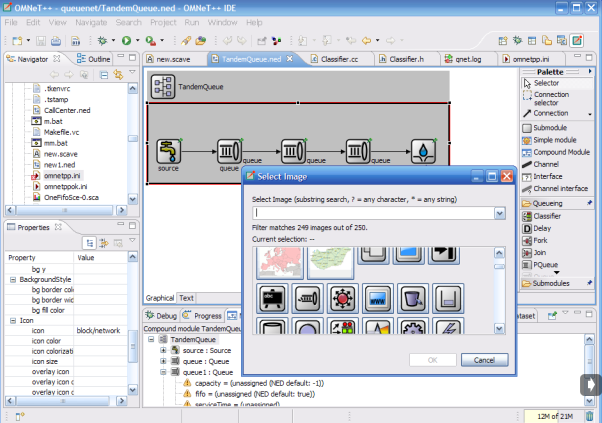
\includegraphics[scale=0.4]{img/omnet}	
\caption{Example of the OMNet++ NED editor IDE }
\end{figure}

\subsubsection{Testbeds}
As an alternative to simulations, testbeds are in-lab networks built and used by researchers, which involves creating and connecting physical devices for testing the application of real networks. As a result, the cost of hardware coupled with the difficulty of managing applications in terms of deployment and monitoring creates limitations on the complexity and scalability of the network. While it can be said that the physical testing environment is much more effective and realistic than a simulation, the lack of larger testbeds of over 50 nodes prevents this from becoming a major component for validating new concepts and applications for MANETs \cite{luchogie2006}.

\subsection{Data Mining and Monitoring}
The core functionality of MANETs is to provide a network of mobile nodes which can communicate with one another and pass information by routing through intermediate nodes where necessary. In a sensor network, each node is tasked with collecting specialised data through the use of sensory peripherals, and this data must be passed effectively to its destination. Given the dynamic nature of MANETS, considerations must be made for the constant changing topology in order to ensure that the networks's integrity and availability is not compromised and that nodes can effectively communicate with one another at any time \cite{ramramathanjasonredi2012}. This includes problems such as losing connection or going out of range, which will cause the loss of packets when communications links are inevitably cut and messages lost. 
Connections between nodes and algorithms for data mining must be carefully established and monitored in order to ensure secure and efficient routing. For example, the data collected by each individual sensor node which is monitoring an environmental feature will typically register similar values due to spatial correlation, so there is a danger for unnecessary overheads as a result of unneeded data. By measuring spatial correlation between data sampled by different sensors, specialised algorithms can be developed to implement more efficient data mining, as well as optimising routing strategies \cite{mayajie2011}. In order to aggregate data more effectively, a  stationary base station node may be included, which acts as the data sink, and may be capable of passing user input to nodes, which would allow for some stability and interaction with the network by the user. 
POSSIBLE OBLIGATORY IMAGE OF BASE STATION NETWORK/BROKEN LINKS

\subsection{Sensor Networks}
A sensor network is different to a simple MANET in that each node has autonomous sensors to monitor physical or environmental conditions such as temperature, sound or pressure. This data can also be routed through other nodes, and it may be possible to control sensor activity if networks are bidirectional \cite{kazem2007}. While sensor networks themselves can range from wired to wireless, or have predefined topologies such as the simple star network or a multi-hop wireless mesh network, a drone sensor network would be classified as a mobile wireless sensor network (MWSN) for obvious reasons. 
The biggest challenges to MWSNs, in general terms, are hardware and environment. Power consumption of the sensing device should be minimised and sensor nodes should be energy-efficient, since their limited energy resource determines their lifetime. As with any mobile network, the varying topology due to the mobility of nodes results in further usage of the already limited resources in terms of battery power. If it is possible, nodes could consider powering off unused parts to save power, such as immediately after takeoff, where sensors may not be required en route to the target area. However, this is also dependent on the environment, which may require additional precautions in the event that it is hazardous or requires heavy monitoring. The most effective method for energy efficiency is the use of optimal routing protocols, which will be discussed in later sections \cite{shiny2012}.

\section{Drones}

\subsection{UAV Components}
As has been discussed in previous chapters, drones have a variety of sizes, utilities, costs, and applications, from commercial to military purposes. However, they will all have to make use of sensors, actuators, software, and a power supply in battery form. The body includes a fuselage and wings for planes, tail rotor for helicopters, and a frame and arms for multirotors \cite{mitchjohnson2015}. The combination of different layers of computer software with different time requirements, also referred to as the autopilot or flight stack, may require specialised externally supported hardware such as Raspberry Pis or Beagleboards. This is because on-board classical operating systems may be too intensive for some embedded systems, presenting problems if the aircraft is dependent on fast response times \cite{paparazzi2016}. 
Depending on its usage, a drone will also range from being fully remotely piloted to complete autonomy such that the drone will function without any user input. Is important to note that the degree of autonomy i.e. the extent to which the aircraft is independent from operator assistance, is different to the level of autonomy in terms of the scope of tasks it can perform and their sophistication \cite{williammarra2012}.

\subsection{Drone Autonomy}
Autonomy is split into different layers of control, from basic manoeuvrability and flight controls to system management, navigation and mission planning. It is assumed that the user will be able to provide task level instructions which the drone is capable of processing. The figure below shows an example of the basic autonomy controls for a UAV.

\begin{figure}
\centering	
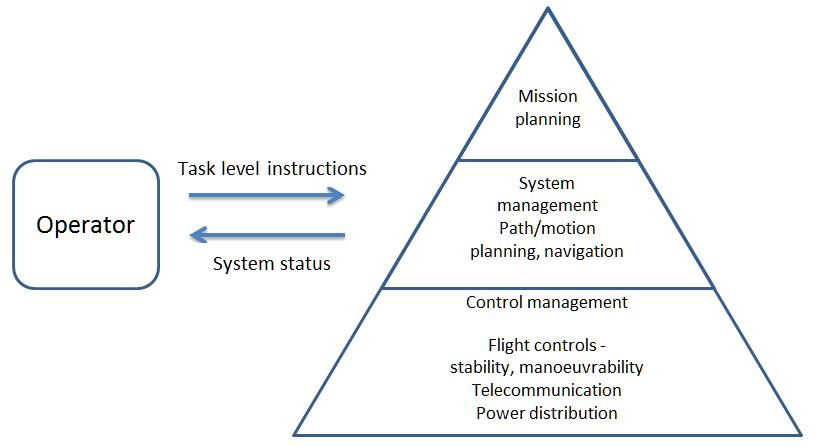
\includegraphics[scale=0.4]{img/autopyra}	
\caption{Hierarchy of drone autonomy and user control}
\end{figure}

An autonomous drone would be expected to have various features for flight control and communications, such as:
\begin{itemize}
\item \textbf{Autonomous takeoff and landing}
\item \textbf{The ability to return to its starting location}
\item \textbf{A failsafe to autonomously land the drone in the event of loss of signal}
\item \textbf{The ability to stabilise and maintain altitude in unstable conditions i.e. hover and self-level in wind}
\item \textbf{Possible GPS waypoint navigation}
\end{itemize}
A drone will already contain a microcontroller with pre-programmed instructions for navigation, including tricks such as rolls and loops; however, an external small computer would be required to implement mid-level algorithms such as those involved in physical routing and communications. For example, determining an optimal path whilst avoiding obstacles, or passing messages in a network to other nodes. The attachment of an external computer such as a Raspberry Pi would allow for the drone to be programmed directly, which is the most common solution achieving autonomy, which will be discussed later.
Reactive autonomy, such as real-time collision avoidance, relies on situational awareness, which is typically provided by range sensors. However, a network of drones with GPS capabilities would be able to utilise its own spatial awareness, knowledge of other node positions and protocols designed to avoid collision. 

\subsection{Classifications}
UAVs have been classified by such areas as weight, functionality, range and usage. Given that this project focuses on the use of consumer-level drones, we will focus on the classification of drones by usage \cite{yashgarg2015}. The fundamental types of drones are as follows:

\begin{itemize}
\item Commercial off-the-shelf (COTS). This refers to drones which are ready to fly immediately with no prior or specialised knowledge required
\item\textbf{ Bind-and-Fly (BNF) and Almost-Ready-to-Fly (ARF).}  BNF and ARF drones typically contain most or only some of the parts required for the drone, but may be missing components such as the controller or battery, and require some knowledge to assemble and configure
\item \textbf{Midsize Military and Commercial Drones.} These drones are more expensive, with greater utilities and/or bespoke functionality
\item \textbf{Large Military-Specific Drones.} Military drones may be used for combat, logistics, research and development, reconnaissance or as target and decoy drones
\item \textbf{Stealth Combat Drones.} Military drones which are used for stealth operations, including direct combat and reconnaissance

\end{itemize}
For a drone sensor network, it is important to be aware of the amount of power consumption, the weight and the range of the drone in order to maximise its efficiency and understand the limitations of the network. COTS drones (or quadcopters) will typically carry a payload (such as a camera), and additional peripherals such as the external computer required for implementing autonomy and sensing equipment will add to the weight of the drone, so considerations must be made for load capacity. Additionally, range will be directly influenced by the choice of medium, such as Wi-Fi or radio. All of these additions to the drone will affect the ‘Degrees of Freedom’, which is the number of axis and sensors combined for balancing a plane, helicopter or robot, which typically is equated with the complexity (and therefore, price) of a UAV \cite{arduinodof2012}.

\section{Existing Solutions}
This chapter has discussed the structure and characteristics of sensor networks, including implementation and testing through simulators, as well as examining different varieties of drones and their components, identifying how this can be related to sensor networks. This section will highlight some of the advances and complications which arise within sensor networks, autonomous drones, and explicit combinations of both, by examining existing implementations and research into the field.

\subsection{Autonomous Drone Implementation}
UAVs and autonomous aircraft have become increasingly popular as an area of research and development, and a number of open source autopilot projects exists which can facilitate autonomy, allowing hobbyists and businesses to use them on small, remotely piloted aircraft inexpensively. Among these are GPS-based projects such as Paparazzi and ArduPilot, which will be analysed to see how they can be applied to drones, and how they differ in terms of their choice of operating system and implementation. Other methods of achieving drone autonomy will also be discussed in this section.

\subsubsection{Paparazzi}
Remes et al. \cite{bartremes13} conducted studies on the use of a GPS-based open source autopilot system known as Paparazzi in order to create a swarm of autonomous Parrot AR drones. The Parrot firmware can be enhanced with Paparazzi firmware, or a standalone version of the Paparazzi firmware can be used. The autopilot will lock onto sufficient GPS satellites, establish a signal and enact a user constructed flight plan.
Paparazzi includes a base station GUI known as the Ground Control Station (GCS) for the purpose of preparation, simulation, monitoring and analysis, and each drone can be located on the map provided.  The overlay includes information about the drones such as height, waypoints for the flight plan and controls. The addition of more drones is arbitrary; installing the firmware on each drone will allow it to be located on the GCS and interacted with. 

\begin{figure}
\centering	
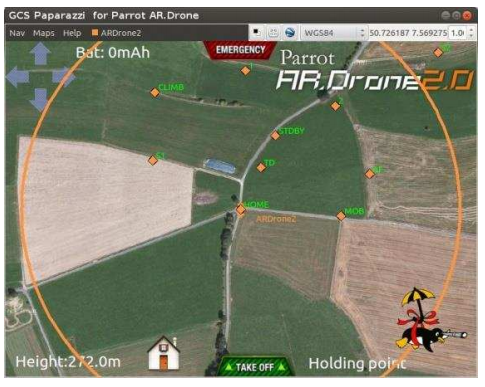
\includegraphics[scale=0.4]{img/papgcs}	
\caption{The Ground Control Station of Paparazzi for the Parrot AR drone 2}
\end{figure}

Both inner and outer loop control is performed by Paparazzi, which means that the flight plan controls the thrust and attitude for achieving the right speed and position, and the safety pilot has control over the vehicle via the RC link, which refers to the joystick connected to the GCS. The control loops are open source, however, and can be changed by the user.

\begin{figure}
\centering	
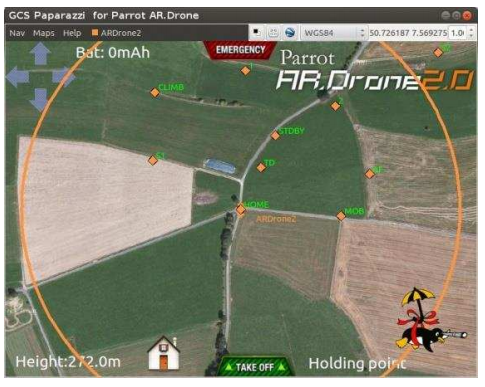
\includegraphics[scale=0.4]{img/papgcs}	
\caption{Global view of the control loops used by the Paparazzi airborne code for navigation, guidance and control}
\end{figure}

\subsubsection{Ardupilot}
He Bin et. al \cite{ hebin2009} discuss the design, modelling, implementation and testing of an autonomous UAV with the use of Ardupilot, which is another open source UAV autopilot platform. Ardupilot is a portmanteau of Arduino and pilot, the open source electronics prototyping platform upon which Ardupilot is based. It is similar to the Paparazzi project in terms of its free software approach and GPS-based implementation. 

\begin{figure}
\centering	
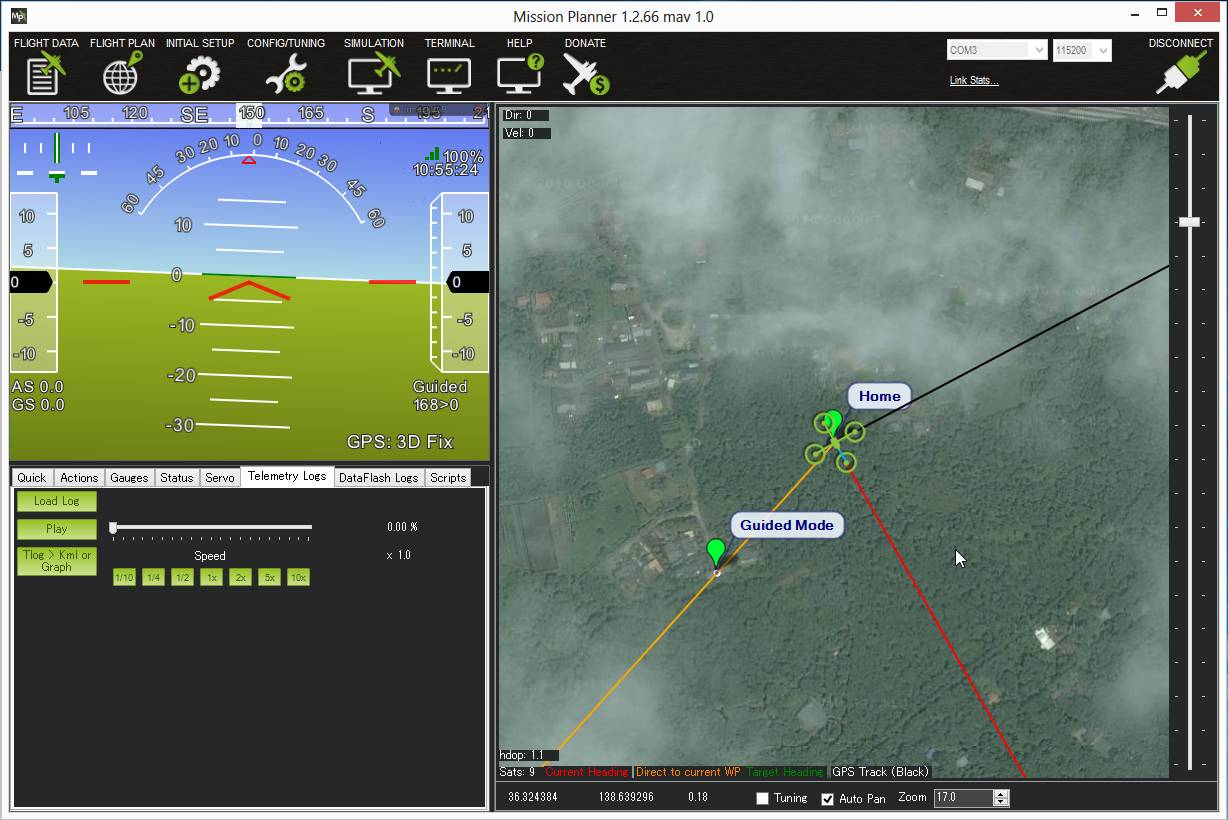
\includegraphics[scale=0.2]{img/ardgui}	
\caption{Example output of  the Ardupilot Mission Planner software}
\end{figure}

The Ardupilot is a custom PCB with an embedded processor combined with a built-in hardware failsafe to switch between RC control and autopilot control, such that the user can decide the amount of direct control over the UAV themselves. The autopilot controls navigation (by following GPS waypoints) and altitude by controlling the rudder and throttle.
The Ardupilot software is an open source Arduino environment which can be easily run and edited on Windows, Mac OS X and Linux, in contrast to Paparazzi, which runs exclusively on Ubuntu, and requires more specialist knowledge (including a reasonable grasp of the command line). However, it requires for waypoints to be set manually and before takeoff, which limits the level of autonomy which can be achieved. Ardupilot is widely regarded as the ‘breakout’ model for autopilots, due to its ease-of-use and price (which is much cheaper than Paparazzi), with somewhat reduced functionality and lower specs.

\subsubsection{Map Stitching}
In order to solve the problem of autonomous drone control, Visser et al. introduce a method of navigation using image stitching to build a visual map of an indoor environment \cite{arnoudvisser2011}. Using the frames from the Parrot AR Drone’s (which we are using for the project) downward-facing camera, sets of matches between two camera frames are used to estimate a tomographic model for the apparent image motion. Thus, a model can be composed with the estimated motion of the rest of the images in order to build a mosaic. Additionally, it makes use of sonar sensor input to detect obstacles, which are then added to the camera image during the image stitching process. An example result of the map stitching is shown in the figure below.

\begin{figure}
\centering	
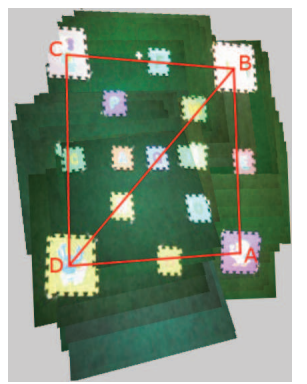
\includegraphics[scale=0.2]{img/mapstitch}	
\caption{Map created by the map stitching method using camera images taken by the AR drone }
\end{figure}

Calculations for frames are further influenced by a number of additional sensors such as inertial sensor data, which can be used to estimate current position, calculate an estimate for the resulting position, and use this as input for the map stitching algorithm. 
**MATHS AND ALGORITHMS HERE?**
Results showed that the visual map created by a simulated AR drone contained fewer errors than a map from the real drone, which could be attributed to the effect of automatic white balancing of the real camera. However, the map stitching method is able to map small areas visually with sufficient quality for human navigation.

\subsubsection{Drone Localisation}
Dijkshoorn et al. \cite{dijkshoorn2011} introduce a similar method for autonomous navigation which uses sensor and motion models to localise an autonomous Parrot AR drone. This method involves creating a visual map using texture and feature mapping derived from the position and attitude of the drone in the world, whereupon the map can be used for absolute position estimates and subsequent navigation. By creating a visual map, it is possible to sufficiently conduct human and artificial navigation through an indoor space. Simulation of the AR drone is also performed to aid in the estimation and testing of localisation methods and mapping.

\begin{figure}
\centering	
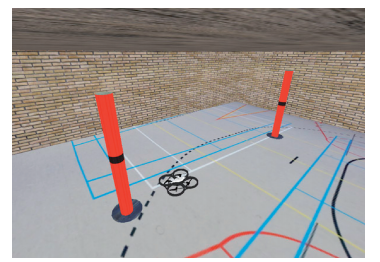
\includegraphics[scale=0.7]{img/dronemod}	
\caption{3D model of a gym with realistic ground and wall textures for AR drone simulation}
\end{figure}

Firstly, to initialise the visual localisation and mapping algorithm, the internal sensors of the drone are used to give information about the position and movement of the drone. The inertial sensor measures body acceleration and angular velocities, which can be converted to an estimated attitude. Sonar sensor is used to measure the altitude of the drone, and an estimation of body velocity is calculated using inertia measurements and optical flow from the relative motion between camera frames. This information is used to build a visual map of the environment.
**MORE MATHS HERE MAYBE**
Results showed that the mapping method is able to map areas visually with sufficient quality for both human and artificial navigation purposes. The simulation contained fewer errors than the real Parrot AR drone, which were attributed to measurement noise, however, the localisation and visualisation methods were demonstrated to make autonomous navigation possible

\subsection{UAV Sensor Networks}

\subsubsection{Collaborative Drone Tasking}
Recognising the difficulty in coordinating multiple drones to perform a task collaboratively in a sensor network, Mottola et al. \cite{mottola2014} introduce and provide an analysis of the concept of team-level programming, which can express collaborative sensing tasks without the complexity of such areas as concurrent programming or parallel execution. They create the VOLTRON programming system to explore this concept and enable coordination of multiple drones with a specific focus on active sensing applications, and dynamic re-tasking.
This method of team-level programming was developed in contrast to drone-level programming and swarm programming, which focus on addressing and tasking each individual drones with navigation, communication and sensing, or executing a single set of basic rules and operating only on their own local state, which is difficult to scale up to multiple drones. Team level programming allows for sophisticated collaborative sensing tasks without resorting to individual addressing, enables simpler code execution and produces marginal overhead in terms of CPU, memory and network utilisation.
Mottola et al. concluded that the implementation of a team-level programming model in VOLTRON provided a significant improvement in execution time for a given task when using multiple drones. Application level performance of real-while drone applications were assumed to depend greatly on hardware design choices and execution times could be variable depending on the environment. Nonetheless, the use of a testbed, as well as real deployment, produced results that VOLTRON does introduce overhead, but that memory consumption and CPU utilisation are independent of the number of drones, and this system would likely scale effectively beyond 100 drones before reaching resource limits. 
**POSSIBLE COMPARISON BETWEEN DIFFERENT IDEAS?/HOW WE FEEL ABOUT THIS**

\subsubsection{Emergency Services}
One of the most common applications of UAVs aside from commercial or military is in the field of disaster prevention, management and relief. Fuego, the Fire Urgency Estimator in Geosynchronous Orbit, is a system created by researchers at UC Berkeley which locates and identifies fires using drones, planes and satellites with special infrared cameras \cite{shelbycarpenter2015}. The network of drones would navigate through fire-prone areas of the country, taking photos at a wavelength of light that fire emits, but which is invisible to the human eye. A geospatial information system (GIS) processes the images in real time to estimate the risk that a hotspot could grow into a serious fire, where the difference in each sample can highlight the eruption of a forest fire. With this system, it is possible to identify forest fires within 3 minutes of their eruption \cite{fuego2015}.
Research into the application of networked UAVs for disaster management is also being conducted to test the ability of small-scale, battery-powered and wirelessly connected UAVs carrying cameras for disaster management, such as a wood fire or a large traffic accident, and deliver high-quality sensor data such as image or video. Quaritsch et al. \cite{quaritsch2010} discuss the potential of the tight integration of sensing and controlling UAVs, which allows for a whole new set of applications and research challenges. Following disasters such as Hurricane Katrina, UAVs were equipped with a digital camera capable of both still and video imagery, for post-disaster data collection and damage inspection of multi-storey commercial buildings \cite{stuartadams2011}. The most prominent challenges to UAV sensor networks are described as optimisation for area coverage, as well as concerns over limited resources, especially energy. Limited site access and landing and takeoff environments also required that there were greater flight distances to reach areas of interest, which further emphasises the importance of energy efficiency. 

\section{Routing}
Two of the biggest challenges for UAV Sensor networks which have been introduced so far are the issues of limited resources and the environment. In order to minimise overheads, reduce computation time, optimise pathing and battery usage, and introduce energy-efficient communication, it is essential to consider different methods of routing in sensor networks. The length of operation time and success of the network relies on firmly established protocols which are optimised for the application. In this section, we examine some of the existing algorithms for routing, giving a brief discussion of the advantages and disadvantages of each method, and how they deal with specific challenges such as robustness and energy efficiency. 

\subsection{Ad Hoc On-Demand Distance Vector}
Ad Hoc On-Demand Distance Vector (AODV) routing is a non-position based protocol which enables dynamic, self-starting, multi-hop routing between participating mobile nodes. It operates by sending Route Request (RREQ), Route Reply (RREP) and Route Error (RERR) messages between nodes, which are used to establish endpoints of a communication connection (as shown in figure \ref{aodv}).  In AODV, the source node and the intermediate nodes store the next top information corresponding to each flow for data packet transmission \cite{perkins2003}.

AODV is a reactive (on-demand) routing protocol in that it does not do anything if an active route already exists between communicating nodes, so connection setup delay is less, and destination sequence numbers are used to find the latest route to the destination. The AODV protocol also keeps the overhead of messages small, and has a great advantage in overhead over simple protocols which need to keep the entire route from source to destination in their messages. This protocol is also loop-free and avoids the counting to infinity problem through the use of sequence numbers. Despite this, such protocols have a high latency time in finding a route (because routing is done in reaction to a message being sent), and excessive flooding can lead to network clogging. 

More information about AODV can be found in section \ref{AODVdesc}.

\begin{figure}
	\centering	
	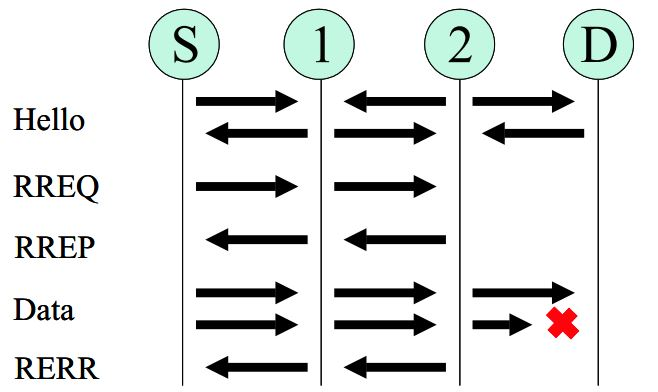
\includegraphics[scale=0.7]{img/aodv}
	\caption{Packet delivery rate for a 50 node model (30 traffic sources)\cite{chakeres2004aodv}}
	\label{aodv}
\end{figure}

\subsection{Dynamic Source Routing}
Like AODV, Dynamic Source Routing (DSR) is an on-demand routing protocol for mobile ad hoc networks. DSR divides the routing problem into two parts: route discovery and route maintenance. Route discovery finds routes between nodes by flooding the network with discovery packets until the destination node is reached. A route reply message is propogated back and cached. Unlike AODV, routes are retained indefinitely (unless they are broken), meaning that when nodes are static the overhead from using DSR is zero\cite{Johnson01dsr:the}\cite{johnson2007dynamic}.

Route maintenance is performed whenever a data message is being sent through the network. Each node is responsible for ensuring that messages it forwards are received (this is often done through link-level protocols or passively on retransmission). In the event of a link being severed and a message being lost, the node which attempted to send over the broken link returns a route error message to the originator of the message. Routes using this link are removed from the cache.

One of the advantages of DSR is that new routes and network updates are retained by every node which witnesses them (each node a route error message passes through will remove the broken link from their routing cache). Additionally, DSR nodes will attempt to shorten routes, salvage packets sent over broken links, and reason about link uni/bi-directionality. This focus on preventing the duplication of messages means that DSR is fast with very low overhead.

\subsection{Greedy Perimeter Stateless Routing}
Greedy Perimeter Stateless Routing (GPSR) take a different approach to routing than AODV and DSR in that it is stateless. Instead of using caching to reduce the amount of overhead, each node memorises the geographical locations of its neighbours and uses this to greedily forward messages. The optimal (one hop) choice for routing is the neighbour which is closest to the destination node\cite{karp2000gpsr} (see figure \ref{gpsr1}).

\begin{figure}
	\centering	
	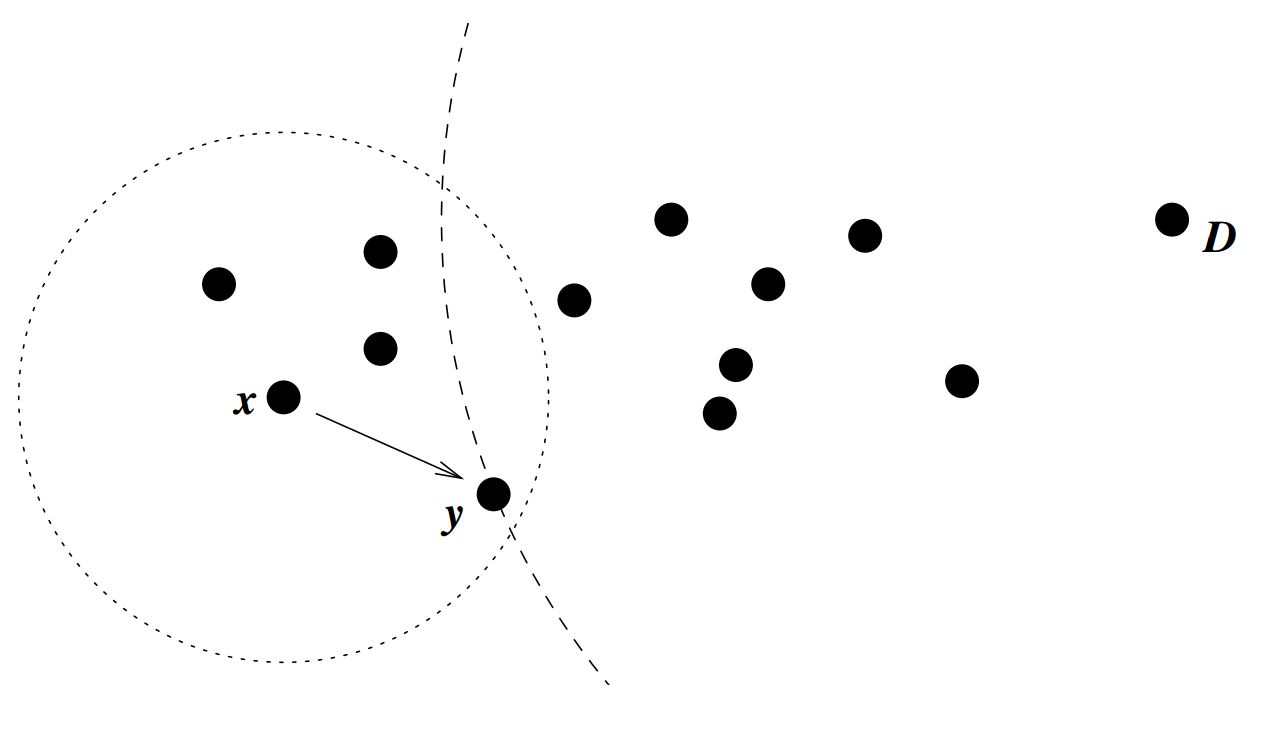
\includegraphics[scale=0.7]{img/gpsr2}
	\caption{An example of greedy forwarding in GPSR\cite{karp2000gpsr}}
	\label{gpsr1}
\end{figure}

The disadvantage of retaining as little information as possible is that there is an associated messaging overhead. GPSR nodes will routinely beacon information about their location, though can be mitigated through the practice of attaching beaconing information to all packets sent. This is exactly what AODV and DSR explicitly try and avoid through the use of caching. There are also scenarios where the optimal node to forward to is not the one chosen by the greedy algorithm. In this case, the right hand rule is used to route packets to their destination.

Benchmark simulations of GPSR and DSR reveal that the overhead incurred by beaconing is normally less than that of more stateful solutions, as shown in figure \ref{gpsr2}. It is worth noting that 

\begin{figure}
	\centering	
	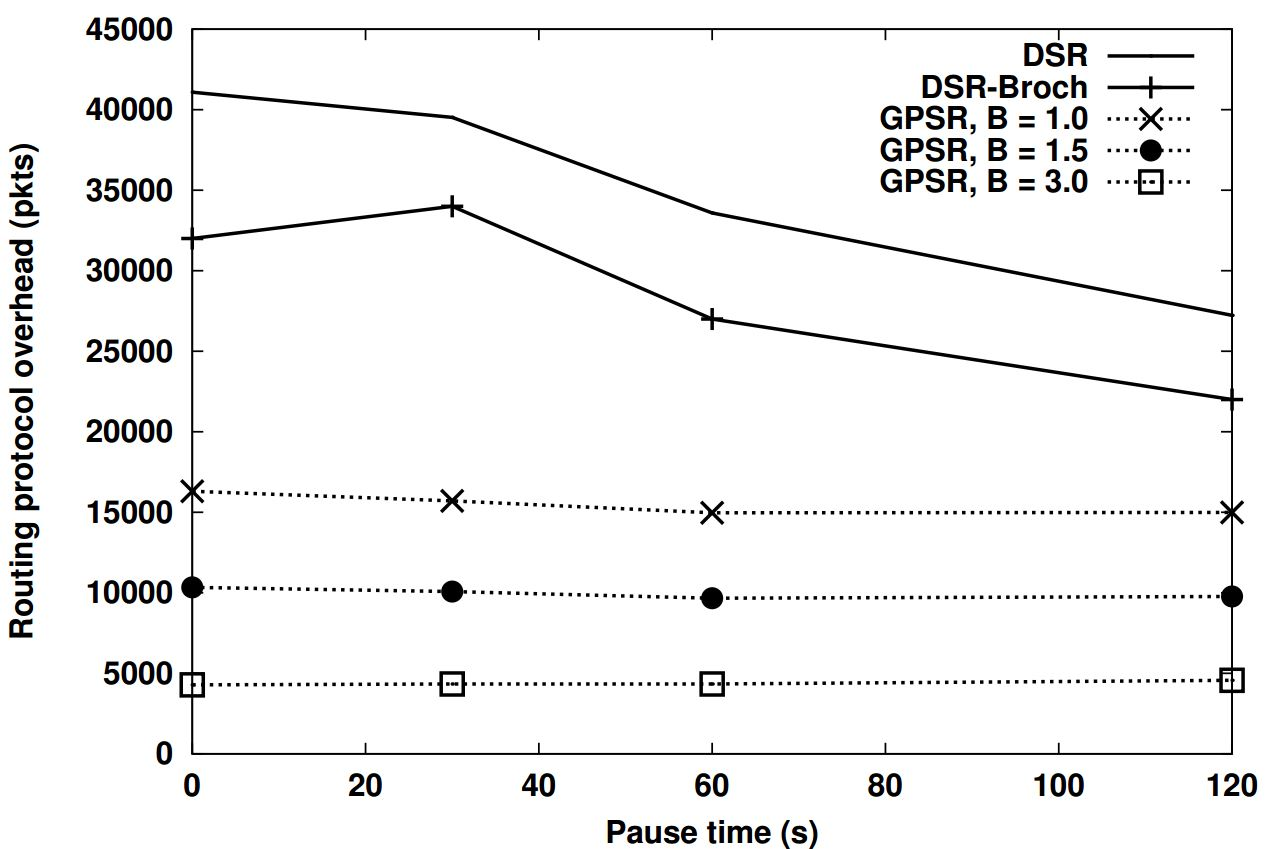
\includegraphics[scale=0.7]{img/gpsr}
	\caption{A comparison between DSR and GPSR with different beaconing intervals $b$\cite{karp2000gpsr}}
	\label{gpsr2}
\end{figure}	
	
\subsection{Comparison}
Figures \ref{dsraodv1}, \ref{dsraodv2}, and \ref{dsraodv3} show a comparison between AODV and DSR in similar conditions. It can be seen that DSR tends to perform better in terms of overhead when considering short pause times (typical of a drone network), but that AODV results in a higher percentage of packets being delivered. Given the need for high priority messages to be delivered as quickly as possible in a quadcopter network (to prevent a collision, for example), it was decided that AODV would be a more appropriate algorithm to implement as a reference communication model in octoDrone than DSR. GPSR is very efficient but suffers from the problem that geographic routing tends to break down when nodes are moving at high speeds most (if not all) of the time. As information on neighbours becomes less certain it is harder to make efficient routing decisions without drastically decreasing the broadcast interval. After some consideration it was decided that AODV would be more broadly applicable, with GPSR being a worthwhile future addition.

\begin{figure}
\centering	
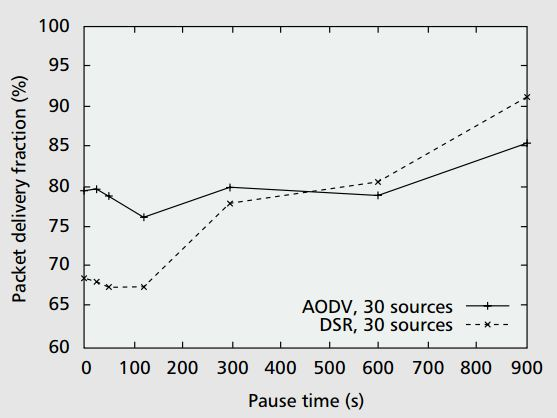
\includegraphics[scale=0.7]{img/comp1}
\caption{Packet delivery rate for a 50 node model (30 traffic sources)\cite{perkins2001performance}}
\label{dsraodv1}
\end{figure}
	
\begin{figure}
\centering	
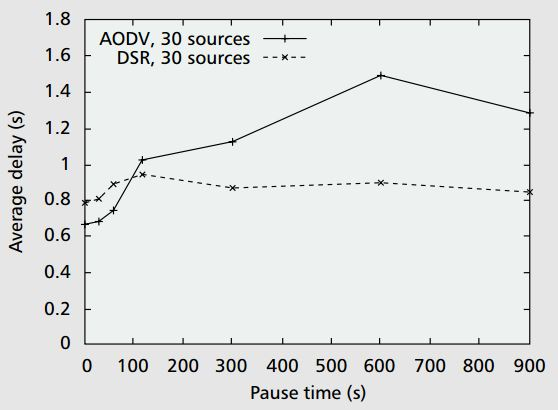
\includegraphics[scale=0.7]{img/comp2}
\caption{Average data packet delay for a 50 node model (30 traffic sources)\cite{perkins2001performance}}
\label{dsraodv2}
\end{figure}
		
\begin{figure}
\centering	
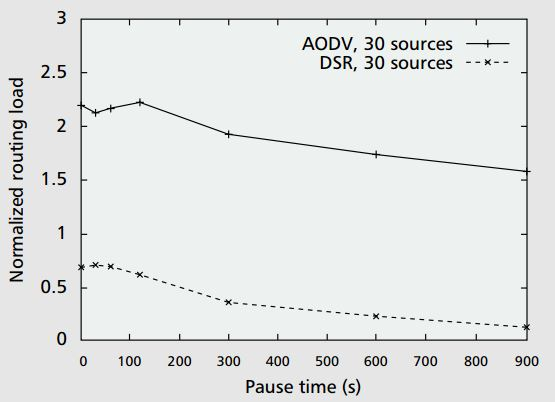
\includegraphics[scale=0.7]{img/comp3}
\caption{Normalised routing load for a 50 node model (30 traffic sources)\cite{perkins2001performance}}
\label{dsraodv3}
\end{figure}
	
\section{Social and Ethical Issues}
The subject of drones has been the focus of much controversy with regards to issues of privacy, invasion of airspace and other unsanctioned uses of UAVs with the ability to, for example, use a camera to take pictures or video. Therefore, a platform for an entire network of drones with a variety of sensors which is open source presents a multitude of possible problems. Furthermore, with the potential to be used as a foundation for military efforts, which form the basis of many current topics of research into drones and sensor networks, there are many implications for potential misuse of the project. As a result, it is necessary to research and discuss the possible methods of unlawful utilisation of drones and drone networks, in order to ensure that the project group is aware of these issues.

\subsection{Privacy}

\subsubsection{Spying}
Freedom of information has been a topic of discussion with regards to the ability to use drones with cameras attached which could be classified as an invasion of privacy. In the UK and the US \cite{rebeccarosen2013}, there has been a huge spike in drone-related incidents, such as drones allegedly flying over peoples’ property repeatedly where they were sunbathing and taking photographs, or hovering in front of the windows of a property with the camera facing inside the window \cite{maryannrusson2015}. It is difficult to argue what constitutes an invasion of privacy, particularly when the law regarding UAVs has yet to be refined in order to reflect the advancement of technology. 
However, the law is very clear with regards to the use of firearms against UAVs, whether or not the UAV in question was trespassing or invading on private property. In November 2014, a man was fined \$850 in damages for shooting down a neighbour’s drone while it was flying over the neighbour's property, and then refusing to pay any compensation for destroying the drone \cite{colinneagle2015}. The Federal Aviation Administration’s (FAA) definition of a drone as aircraft also means that, technically, shooting a drone could result in a maximum penalty of a 20 year prison sentence. Pursuing legal action in cases such as this is difficult, as it is not illegal to fly a drone in public.

\subsubsection{Data Collection}
A more prevalent issue arises where any drone carrying a payload such as a camera has the potential for recording data unlawfully. In one instance, a drone which was found to be hovering over an ATM that seemed to be recording people entering their pin numbers into a cash machine. It can be argued that the drone was not breaking the law by simply recording a public space\cite{maryannrusson2015}. However, it is difficult to prove that the usage of the drone was for the express purpose of obtaining peoples’ pin number, or if this is unlawful to begin with, in the same way that there is no law which expressly forbids someone from looking over the shoulder of an ATM user.
A full-length documentary called Speciesism: The Movie based its foundational discoveries and source of information by using drones to spy on factory farms and record evidence of environmental damage, and went on to feature major global press coverage. In this particular instance, the law with regards to prosecution was unclear, despite the activity being labelled as ‘spying’. This could suggest that such uses of drones, even on potentially private property, may not be possible to prosecute, although this may be unique to incidences of whistleblowing.
** PICTURE OF SPYING IMAGE?**

\subsubsection{Unsanctioned Airspace}
There are several instances where the misuse of drones has been well established and prosecuted. In the very first case of prosecution against unsanctioned drone usage, a security guard was sentenced after repeatedly flying drones over and around Premier league football stadiums, Buckingham Palace and Parliament buildings, where he was fined and banned from flying UAVs \cite{maryannrusson2015}.  In the US, FAA regulations state that drones must not be flown near airports and other areas with manned aircraft, as well as placing a ban on altitudes over 400ft. The Civil Aviation Authority (CAA) in the UK states that for a Small Unmanned Surveillance Aircraft (SUAS) of less than 20 kg, the operation must not endanger anyone or anything, and the aircraft must be within visual line of sight \cite{civilaviationauthority2015}.
For the specific case outlined above, the aircraft being used for surveillance purposes was in violation of the rules of direct line of sight of the aircraft, as well as being subjected tighter restrictions with regard to the minimum distances that you can fly near people properties that are not under control. In most instances of prosecution, the owner of the drone would be required to have permission from the CAA to fly their drone in that airspace, which is in an area that would usually be forbidden access.

\subsection{Military Use}
As discussed in previous sections, engaging in military operations is one of the most prevalent uses for drones, as well as being a popular area for research and development of UAVs. Fortunately, the specs of consumer-level drones are not of a high enough calibre to warrant usage in the military, which requires state-of-the-art hardware, including weaponry. However, there is an initiative to create small, hand-sized mini drones for soldiers in the US Army, for the purpose of small scale intelligence gathering and reconnaissance, in place of conventional air support \cite{jonfingas2016}. Project such as this have implications for the usage of drones of all shapes and sizes in military operations, which would suggest that implementations of drone autonomy by hobbyists and businesses may form a basis for research and development in the army.
The use of drones for spying is not only limited to consumers, as the military has also been responsible for deploying drones to spy on civilians in their home country. The Department of Defense in the United States has admitted to using Predator and Reaper military drones in the US since 2006 in order to support domestic civil authorities, which was made public in March 2016 \cite{pentagon2016}. According to the government, these domestic drone flights are stated as not being in violation of any laws, and were being employed in a “very, very minimal way, very seldom”.

\subsubsection{Other Illegal or Unsanctioned Use}
There have also been cases of the use of drones in order to smuggle illegal substances into high security areas. Scotland Yard has logged various different drone-related incidents, including complaints about drones being used to ferry drugs into prison \cite{maryannrusson2015}.  It is highly likely that an individual or individuals would be responsible for such use of drones, particularly in violation of multiple laws \cite{civilaviationauthority2015}, as opposed to commercial businesses. However, this implies that open source autopilot software and other similar platforms may be used unlawfully by individuals.
